\documentclass[12pt,french,titlepage]{article}
\usepackage[utf8]{inputenc}
\usepackage{geometry}
\usepackage{amsfonts}
\usepackage{float}
\usepackage{graphicx}
\usepackage{hyperref}
\hypersetup{colorlinks,urlcolor=blue}
\geometry{
 a4paper,
 left=25mm,
 right=25mm,
 top=25mm,
 bottom=25mm
 }
\title{\textbf{Game of Thrones} \\ House of D2SI}
\date{\vspace{-35ex}}
\begin{document}

\maketitle

\section{Contexte}

Aemon, maester de Castle Black, est l'un des plus proches conseillers de Lord Commander Jeor Mormont. Il est aussi le dirigeant de la bibliothèque de Castle Black qui contient des centaines de milliers de livres dont certains que l'on ne trouve nulle part ailleurs dans les sept royaumes, pas même dans la Citadelle.
\\\\
Chercher de l'information dans cette bibliothèque immense est un véritable challenge, et au fur et à mesure que les années passent cette tâche devient de plus en plus fastidieuse pour Aemon. Il fait donc appel à Sam, son apprenti préféré, et lui demande de trouver une méthode qui va lui permettre de \textbf{trouver facilement une information à partir de mots clefs}. Sam demande à son tour de l'aide à son ami Jon Snow qui a toujours eu un faible pour la recherche d'information et le data engineering. 
\\
Jon Snow décide alors d'utiliser une représentation vectorielle de document.
\\\\
Pour cet exercice, nous nous mettons dans la peau de Jon Snow pour implémenter de manière efficace la construction d'un \textbf{index inversé}. Souvenez-vous, la bibliothèque de Castle Black contient beaucoup de livres, le jeu de données fourni n'en est qu'une petite partie et votre implémentation doit tenir compte de cette contrainte.

\section{Algorithme}

Dans le domaine de la recherche d'information, les documents peuvent être représentés de plusieurs manière, et notamment de manière vectorielle. Une représentation vectorielle a pour avantage de donner un accès direct à des outils mathématiques tels que la distance, la similarité, la réduction de dimensions, etc...
\\\\ 
Notre exercice ne concerne pas directement ces outils mathématiques mais il s'agit de créer un index inversé des documents afin d'accélérer les calculs. En effet ceux-ci s'appuient souvent sur des produits scalaires qui sont coûteux en calcul et en mémoire. Le calcul des produits scalaire est simplifié lorsque l'on dispose d'un index inversé.

\subsection{Index inversé}
\paragraph{Hypothèse}Nous avons une collection de documents de taille N. Dans notre cas nous avons un fichier par document et le nom du fichier est simplement l'indice du document (1,2,3,...)
\begin{figure}[H]
    \centering
    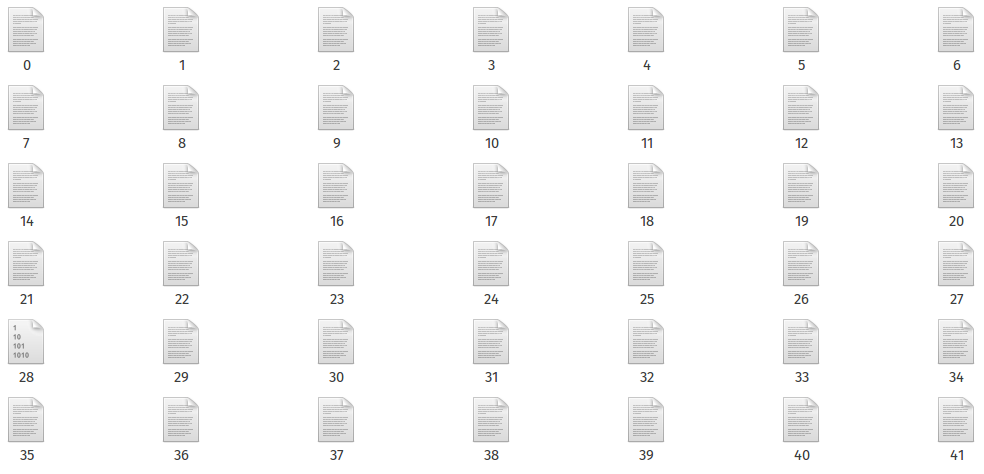
\includegraphics[scale=0.45]{images/corpus}
    \caption{Collection de documents}
\end{figure}
Nous avons également un dictionnaire de taille M associant chacun des mots du corpus mot à un indentifiant unique.
\begin{figure}[H]
    \centering
    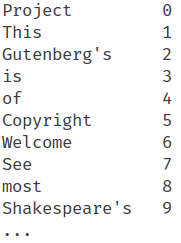
\includegraphics[scale=0.75]{images/dictionnaire}
    \caption{Exemple de dictionnaire}
\end{figure}

Cela va nous permettre de construire un index inversé qui pour chaque mot fournit l’ensemble des documents dans lesquels il apparaît.

\begin{figure}[H]
    \centering
    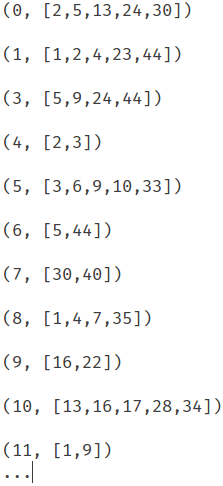
\includegraphics[scale=0.6]{images/index_inverse}
    \caption{Exemple d'index inversé}
\end{figure}

\subsubsection{Construction de l'index inversé}

Notre solution doit fonctionner dans le cas d'un très grand corpus de documents. Notre algorithme doit pouvoir tourner sur un système distribué de plusieurs noeuds afin de ne pas être limité par le stockage, la puissance et la mémoire d'une seule machine. 
\\\\
Notre algorithme se fera en 4 étapes.
\begin{enumerate}
    \item Collecter l'ensemble des paires (idMot, idDoc)
    \item Trier ces paires par ordre idMot puis idDoc
    \item Grouper ces paires pour chaque idMot, afin d'avoir la liste des docs pour chaque mot
    \item Fusionner les index inversés intermédiares pour obtenir l'index inversé final
\end{enumerate}

\begin{figure}[H]
    \centering
    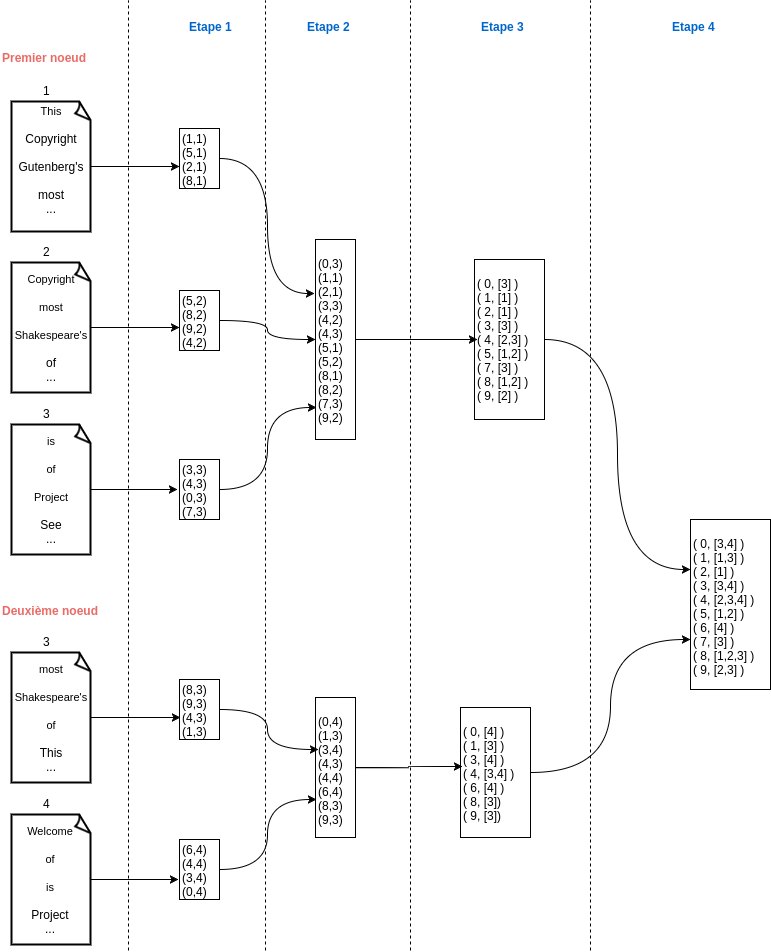
\includegraphics[scale=0.6]{images/algorithme}
    \caption{Illustration de l'algorithme}
\end{figure}

\textbf{N.B:} L'index inversé doit être trié par ordre des identifiants des mots et chaque liste d'une entrée doit être triée par ordre des identifiants des documents.

Algorithme associé: \href{https://nlp.stanford.edu/IR-book/html/htmledition/blocked-sort-based-indexing-1.html}{\underline{Blocked sort-based indexing}}

\section{Questions}

Nous fournissons un corpus de documents disponible dans le dossier corpus de dépôt.

\paragraph{1.} Implémenter un job pour construire le dictionnaire. Dans les documents, les mots sont séparés par un ou plusieurs espaces. Une ligne de ce dictionnaire contiendra le mot et son identifiant.

\paragraph{2.} Implémentez la construction de l'index inversé en un ou plusieurs jobs.
\newline
\newline
Vous avez le choix entre les outils Hadoop et Spark pour l'écriture de ces jobs, dans le langage de votre choix.

\end{document}
